\chapter{Supporting controls and implementation details}
\label{app:controls}
These experiments remain part of the evidence. They are grouped here so that the main results chapter follows the argument from controlled order effects to real search, stronger baselines and scheduling robustness.

\section{Contiguous runs, alignment, and placement quality}
Figure~\ref{fig:runs} separates hit-fraction behaviour from cycle behaviour. To summarise hit saturation on the finite grid, the threshold is the smallest tested run length for which that point and every larger tested point are within one percentage point of the best hit fraction in the same width/offset sweep. Table~\ref{tab:threshold} reports the resulting run \emph{bytes}. This is an empirical finite-grid summary, not a physical-law fit or a guarantee about untested run lengths.

\begin{figure}[htbp]\centering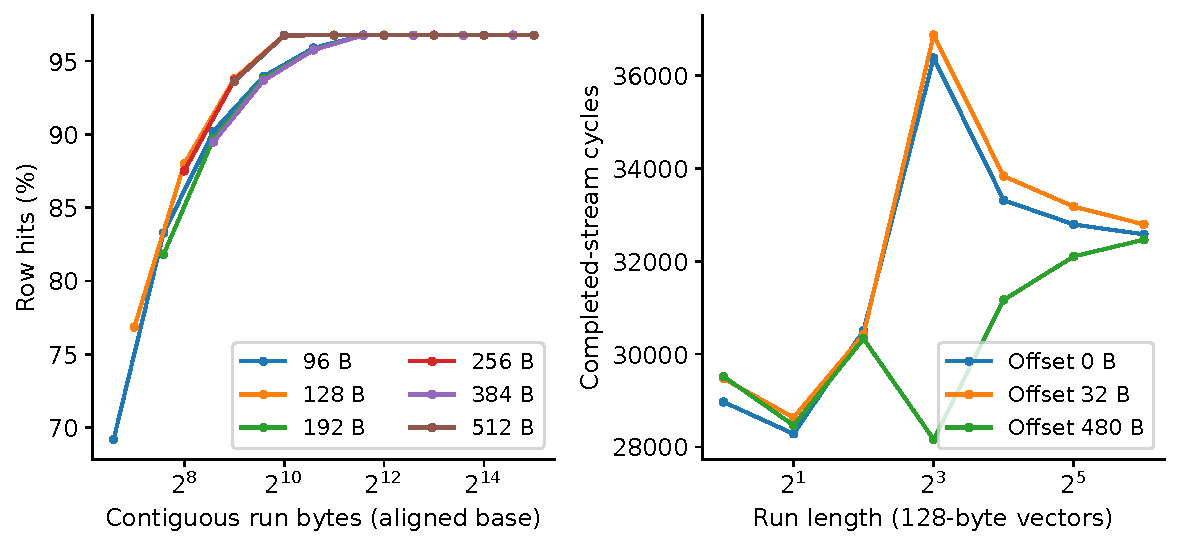
\includegraphics[width=\textwidth]{generated/run_sensitivity.pdf}
\caption[Contiguous runs and alignment]{Contiguous-run sensitivity to payload width and alignment. The left panel measures classified hits; the right panel shows that cycle behaviour requires separate examination.}\label{fig:runs}\end{figure}
\begin{table}[htbp]\centering\caption[Empirical run-byte thresholds]{Run-byte threshold for sustained hit fraction within one percentage point of the best tested point, by base offset. The threshold is conditional on this grid and configuration.}\label{tab:threshold}
\begin{tabular}{lrrr}
\toprule
Vector bytes & Offset 0 & Offset 32 & Offset 480 \\
\midrule
96 & 1536 & 3072 & 3072 \\
128 & 1024 & 4096 & 4096 \\
192 & 1536 & 3072 & 3072 \\
256 & 1024 & 4096 & 4096 \\
384 & 3072 & 3072 & 3072 \\
512 & 1024 & 4096 & 4096 \\
\bottomrule
\end{tabular}
\end{table}

The 1-KiB contiguous row span is independently established by address decoding. A saturation threshold can be larger, smaller in a particular grid, or affected by alignment and the controller's request mix. It should not be used to infer the row size after the fact. The alternate mapping experiments additionally change the bank opportunities associated with a contiguous address range. A predictive universal byte-budget rule is not established.

Figure~\ref{fig:quality} and Table~\ref{tab:quality} use only bijective layouts with identical address multisets. Reducing the fixed-slot fraction can move a vector within or across its original bank-row group, so the percentage is not a direct measurement of retained row locality. The curve describes this chosen corruption process. The experiment measures robustness to this specific perturbation. Translating a fixed-slot percentage into an acceptable engineering threshold would require a target cycle benefit and a preprocessing-cost model.
\begin{figure}[htbp]\centering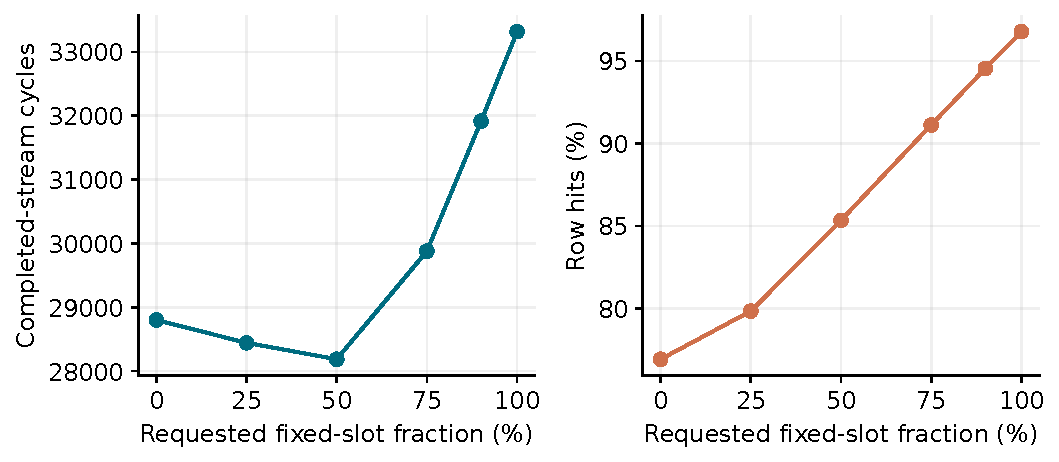
\includegraphics[width=\textwidth]{generated/quality.pdf}
\caption[Placement perturbation]{Valid fixed-slot-quality experiment. Each condition retains all 4,096 storage slots exactly once.}\label{fig:quality}\end{figure}
\begin{table}[htbp]\centering\caption[Placement-quality measurements]{Placement-quality results under the specified cyclic displacement process.}\label{tab:quality}
\begin{tabular}{lrr}
\toprule
Fixed slots (\%) & Cycles & Hit (\%) \\
\midrule
0 & 28801 & 76.92 \\
25 & 28443 & 79.84 \\
50 & 28186 & 85.34 \\
75 & 29880 & 91.11 \\
90 & 31915 & 94.54 \\
100 & 33316 & 96.77 \\
\bottomrule
\end{tabular}
\end{table}

\clearpage
\section{Controller and heuristic sensitivity}
\label{app:exploratory}
Figure~\ref{fig:sensitivity} compares layouts under the one-setting-at-a-time controller matrix. Each cell is a relative cycle difference against BFS in the \emph{same} condition and split. The heat map should not be read as independent evidence from ten repetitions for each cell. It shows how a finding can change when the issue model or bank mapping changes.

\begin{figure}[p]\centering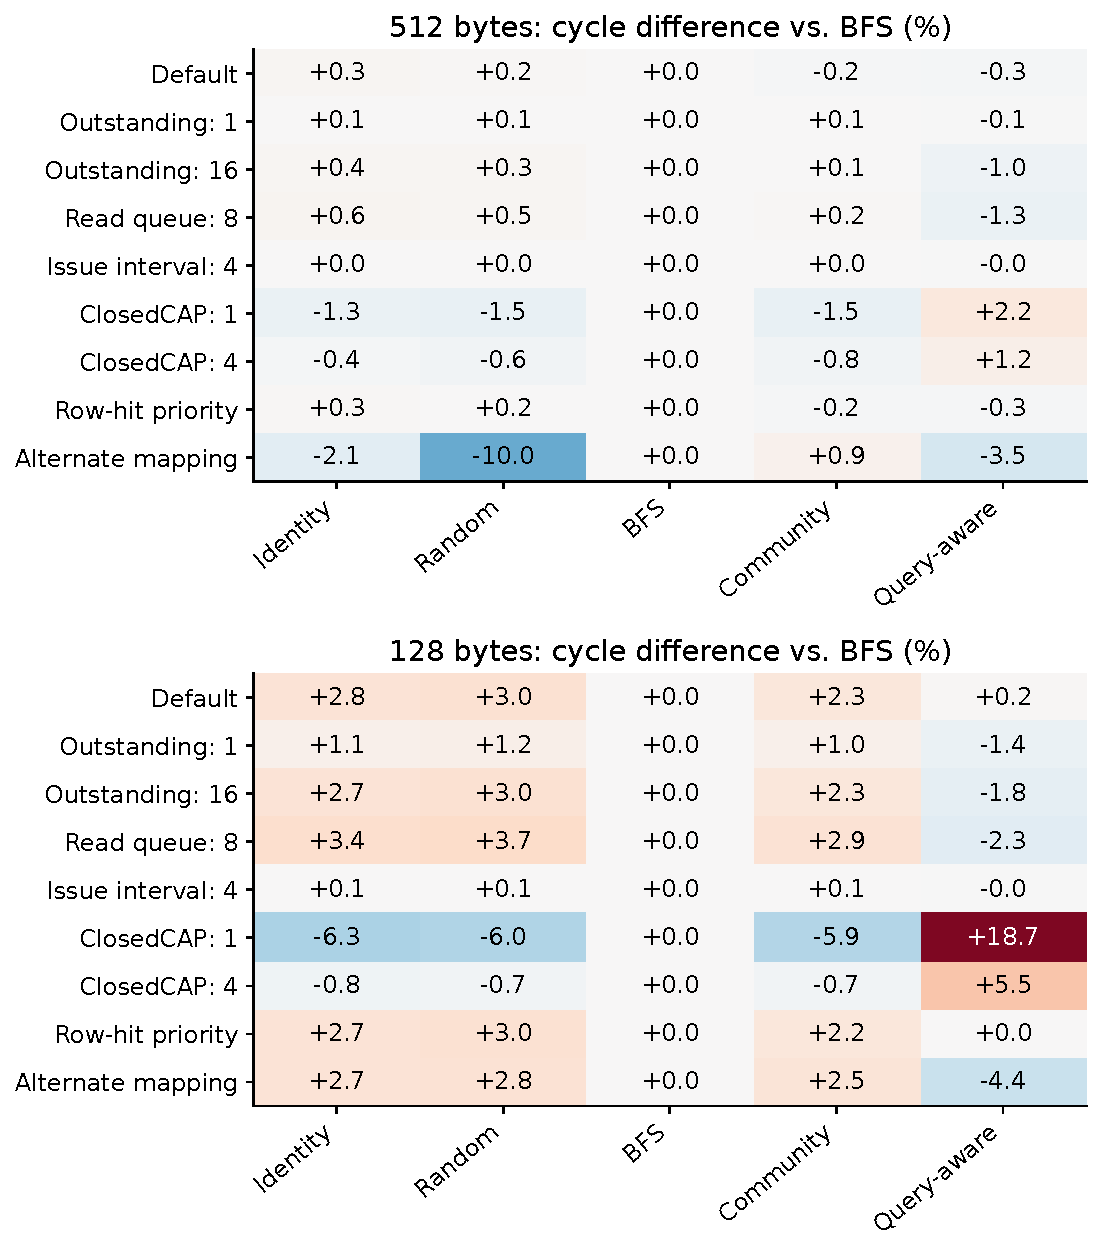
\includegraphics[width=\textwidth]{generated/sensitivity.pdf}
\caption[Exploratory controller sensitivity]{Split-one controller sensitivity. Values are cycle differences in percent against BFS; negative is fewer cycles. The two footprints use separately rebuilt layouts.}\label{fig:sensitivity}\end{figure}

The sensitivity matrix reverses some layout comparisons. For example, the workload-trained layout is faster than BFS with one outstanding request at both footprints, but slower under both capped policies. The alternate mapper favours it relative to BFS at both footprints in this split, although random placement is faster still for 512-byte vectors. These observations show dependence on the memory model; they are not additional ten-split estimates.

The cap-one policy and cap-four policy are explicitly different. In the controlled ordering traces, cap one gives sequential 146,441 cycles and random 33,798 cycles, while their classified hit fractions remain close to 50\%; cap four gives 63,333 and 29,708 cycles. These counters follow the simulator's scheduling-time classification and must not be interpreted as a guarantee that cap one produces zero classified hits. The much larger cycle separation demonstrates why a page-policy label or hit fraction is insufficient to predict service. The real-layout matrix supplies the relevant direct comparison; no claim that all placement benefit requires an open-page controller follows from the synthetic pair alone.

The ablations also change the sign of the comparison: the four-entry history loses to BFS at both widths, while 1,000 training queries give the workload-trained layout fewer cycles at both widths in this split. More training is not uniformly better for every footprint. These tests support examining the heuristic's objective and capacity rather than attributing all performance to static graph locality.

Table~\ref{tab:ablations} changes the heuristic's training and grouping parameters while retaining the test queries. Mean test vector-access coverage by the default training set is \MeanCoverage\%. Coverage here counts accesses whose node appeared in training, not the fraction of all corpus nodes or the fraction of learned edges shared with the graph. The ablations can reveal a limitation of this heuristic, but do not establish why every possible workload-trained placement would succeed or fail.

\begin{table}[htbp]\centering\small\caption[Training and grouping ablations]{Split-one heuristic ablations. Coverage is the fraction of test vector accesses to a node seen in training; model time excludes search collection and layout construction.}\label{tab:ablations}
\begin{tabular}{lrrrr}
\toprule
Condition & Bytes & $\Delta$ QA/BFS (\%) & Coverage (\%) & Model (s) \\
\midrule
train100 & 512 & -0.53 & 71.2 & 1.737 \\
train100 & 128 & +0.76 & 71.2 & 1.737 \\
train1000 & 512 & -0.26 & 99.7 & 24.494 \\
train1000 & 128 & -0.11 & 99.7 & 24.494 \\
window4 & 512 & +0.57 & 97.6 & 2.565 \\
window4 & 128 & +0.93 & 97.6 & 2.565 \\
window64 & 512 & -0.39 & 97.6 & 48.466 \\
window64 & 128 & +0.25 & 97.6 & 48.466 \\
block2048 & 512 & +0.24 & 97.6 & 11.249 \\
block2048 & 128 & +0.49 & 97.6 & 11.249 \\
\bottomrule
\end{tabular}
\end{table}


\section{Published-layout adapter and equivalence checks}
\label{app:adapters}
The source archive and extracted headers are hash-pinned. The adapter retains the supplied score updates and window-expiration condition \texttt{i > w+1}; that condition leaves the initial seed's contribution in place as later nodes expire. We report the supplied implementation rather than silently changing it to an idealised window. To make its weighted queue tractable at 100,000 nodes, an ordered set replaces the linked-list queue while preserving float score arithmetic and update-recency tie order. All three methods give byte-identical permutations to the untouched reference on 30 deterministic weighted test graphs (90 comparisons). This is a differential implementation check, not a proof for every possible graph. Timed preprocessing belongs to this adapted implementation.

\section{Scheduling: service variation within each case}
\label{app:scheduling-detail}
Table~\ref{tab:scheduling-query} supplements the total-cycle comparisons with original-query service. Positive saved cycles mean a reduction; negative percentile differences mean a lower empirical tail. Ranges cover the ten split-level summaries, rather than an interval estimated by treating all query records as independent. Complete paired effects for both sorted and round-robin orders remain in \texttt{results/scheduling\_pairs.csv} and \texttt{results/scheduling\_summary.csv}.

\begin{table}[htbp]\centering\small
\caption[Scheduling sensitivity by original query]{Round-robin versus matching original-order BFS. Saved cycles/query are averaged across ten splits; faster-query fractions and empirical 95th-percentile changes show the observed split range. Original-query intervals include inter-phase and inter-batch gaps.}\label{tab:scheduling-query}
\resizebox{\textwidth}{!}{\begin{tabular}{lrrrr}
\toprule
Condition & Bytes & Saved cycles/query & Faster queries (\%) & p95 change (\%) \\
\midrule
Default (64 outstanding) & 512 & +5,802 & 100.0--100.0 & -15.24 to -13.76 \\
Default (64 outstanding) & 128 & -541 & 6.0--15.0 & +4.25 to +5.95 \\
16 outstanding & 512 & +20,418 & 100.0--100.0 & -33.12 to -31.09 \\
16 outstanding & 128 & +2,106 & 100.0--100.0 & -11.09 to -9.00 \\
32 outstanding & 512 & +9,646 & 100.0--100.0 & -22.63 to -21.29 \\
32 outstanding & 128 & -261 & 20.5--31.0 & +0.63 to +3.86 \\
128 outstanding & 512 & +5,802 & 100.0--100.0 & -15.24 to -13.76 \\
128 outstanding & 128 & -541 & 6.0--15.0 & +4.25 to +5.95 \\
Candidate batches of 2 & 512 & +5,644 & 100.0--100.0 & -8.25 to -7.40 \\
Candidate batches of 2 & 128 & +559 & 92.5--96.0 & -2.54 to -1.11 \\
Candidate batches of 8 & 512 & +7,176 & 100.0--100.0 & -17.25 to -15.18 \\
Candidate batches of 8 & 128 & +500 & 87.0--95.0 & -3.59 to -1.72 \\
Alternative address mapping & 512 & -121,795 & 0.0--0.0 & +144.65 to +159.38 \\
Alternative address mapping & 128 & -25,309 & 0.0--0.0 & +56.29 to +59.74 \\
\bottomrule
\end{tabular}
}
\end{table}

\section{Calibration service and held-out savings}
\label{app:profile-cost}
Table~\ref{tab:profile-cost} reports the memory service spent on all three 50-query calibration runs, averaged over ten splits. The saving per held-out query uses the selected order and matching original-order BFS, including every phase gap. These figures share simulator units, but omit the operations and overlap of an actual execution. They therefore support a service-cost comparison, not a real deployment break-even calculation. Zero or negative held-out saving cannot pay for calibration in this simple accounting.

\begin{table}[htbp]\centering\small
\caption[Profiling cost and service saving]{Mean calibration service for 150 query replays per configuration, and mean saved cycles per held-out query relative to matching original order. Positive saved cycles are favourable. Calibration is performed once per profile; its reuse lifetime is unmeasured.}\label{tab:profile-cost}
\resizebox{\textwidth}{!}{\begin{tabular}{lrrr}
\toprule
Condition & Bytes & Calibration cycles & Saved cycles/query \\
\midrule
Default (64 outstanding) & 512 & 5,716,851 & +5,802 \\
Default (64 outstanding) & 128 & 2,404,776 & +0 \\
16 outstanding & 512 & 8,299,167 & +20,418 \\
16 outstanding & 128 & 2,895,259 & +2,106 \\
32 outstanding & 512 & 6,175,037 & +9,646 \\
32 outstanding & 128 & 2,440,817 & +0 \\
128 outstanding & 512 & 5,716,851 & +5,802 \\
128 outstanding & 128 & 2,404,776 & +0 \\
Candidate batches of 2 & 512 & 10,671,837 & +5,644 \\
Candidate batches of 2 & 128 & 5,652,508 & +559 \\
Candidate batches of 8 & 512 & 6,606,104 & +7,176 \\
Candidate batches of 8 & 128 & 3,025,606 & +500 \\
Alternative address mapping & 512 & 22,547,707 & +0 \\
Alternative address mapping & 128 & 10,246,779 & +202 \\
\bottomrule
\end{tabular}
}
\end{table}

\begin{table}[htbp]\centering\small
\caption[Per-query effects of the selected path]{Training-selected schedule versus matching original-order BFS. Entries show the range across ten splits of the fraction of queries with greater service time and the empirical 95th-percentile difference. Zero in a case selecting original order denotes the identical stream, not a separate confirmation of equivalence.}\label{tab:profile-query}
\resizebox{\textwidth}{!}{\begin{tabular}{lrrr}
\toprule
Condition & Bytes & Slower queries (\%) & p95 change (\%) \\
\midrule
Default (64 outstanding) & 512 & 0.0--0.0 & -15.24 to -13.76 \\
Default (64 outstanding) & 128 & 0.0--0.0 & +0.00 to +0.00 \\
16 outstanding & 512 & 0.0--0.0 & -33.12 to -31.09 \\
16 outstanding & 128 & 0.0--0.0 & -11.09 to -9.00 \\
32 outstanding & 512 & 0.0--0.0 & -22.63 to -21.29 \\
32 outstanding & 128 & 0.0--0.0 & +0.00 to +0.00 \\
128 outstanding & 512 & 0.0--0.0 & -15.24 to -13.76 \\
128 outstanding & 128 & 0.0--0.0 & +0.00 to +0.00 \\
Candidate batches of 2 & 512 & 0.0--0.0 & -8.25 to -7.40 \\
Candidate batches of 2 & 128 & 4.0--7.5 & -2.54 to -1.11 \\
Candidate batches of 8 & 512 & 0.0--0.0 & -17.25 to -15.18 \\
Candidate batches of 8 & 128 & 5.0--13.0 & -3.59 to -1.72 \\
Alternative address mapping & 512 & 0.0--0.0 & +0.00 to +0.00 \\
Alternative address mapping & 128 & 20.5--28.0 & -0.68 to +0.38 \\
\bottomrule
\end{tabular}
}
\end{table}

Table~\ref{tab:profile-service} provides absolute service means across all seven configurations. It prevents a favourable percentage against a slower configuration-specific baseline from being mistaken for a faster overall configuration. Lower outstanding capacity and smaller batches change the original-order service time as well as the gain from scheduling. The measured times still omit the computation and buffer constraints that would decide a deployed configuration.

\begin{table}[htbp]\centering\small
\caption[Absolute service across execution configurations]{Original and training-selected BFS service per held-out query, averaged across ten splits. Only the named setting changes from the default. These are simulated service means, not application latencies.}\label{tab:profile-service}
\resizebox{\textwidth}{!}{\begin{tabular}{lrrr}
\toprule
Condition & Bytes & Original cycles/query & Selected cycles/query \\
\midrule
Default (64 outstanding) & 512 & 39,811 & 34,008 \\
Default (64 outstanding) & 128 & 15,768 & 15,768 \\
16 outstanding & 512 & 61,734 & 41,316 \\
16 outstanding & 128 & 19,853 & 17,747 \\
32 outstanding & 512 & 44,116 & 34,471 \\
32 outstanding & 128 & 16,095 & 16,095 \\
128 outstanding & 512 & 39,811 & 34,008 \\
128 outstanding & 128 & 15,768 & 15,768 \\
Candidate batches of 2 & 512 & 72,625 & 66,981 \\
Candidate batches of 2 & 128 & 37,662 & 37,103 \\
Candidate batches of 8 & 512 & 46,150 & 38,974 \\
Candidate batches of 8 & 128 & 20,197 & 19,697 \\
Alternative address mapping & 512 & 108,034 & 108,034 \\
Alternative address mapping & 128 & 59,417 & 59,215 \\
\bottomrule
\end{tabular}
}
\end{table}
